\section{Placement Results}
\label{sec:results}

Here, we present test results for a basic SA placer as well as test results for four simple variations as listed below. 
Note that midpoint simply means centroid.

\begin{itemize}
    \item \texttt{PlacerGreedyRandom}: all undirected random moves with greedy acceptance
    \item \texttt{PlacerGreedyMidpoint}: all directed centroid moves with greedy acceptance
    \item \texttt{PlacerAnnealRandom}: all undirected random moves with annealing acceptance \textbf{(the basic SA algorithm)}
    \item \texttt{PlacerAnnealMidpoint}: all directed centroid moves with annealing acceptance
    \item \texttt{PlacerAnnealHybrid}: 50\% random - 50\% centroid moves with annealing acceptance
\end{itemize}

We will need an HDL design that utilizes a good mixture of LUTs, FFs, BRAMs, and DSPs at scale to demonstrate the robustness and performance of our placers. 
Any DSP subsystem can serve as a good candidate for such a demonstration. 
Here, we will perform placement on a 2048th-order FIR Filter which was conveniently created as coursework for a VLSI course. 
After passing synthesis, the FIR Filter design calls for the following primitive cells:
\begin{itemize}
    \item 1693 \texttt{LUT} (1-6)
    \item 920 \texttt{FDRE} + \texttt{FDSE}
    \item 282 \texttt{CARRY4}
    \item 32 \texttt{RAMB48E1}
    \item 64 \texttt{DSP48E1}
\end{itemize}

We will perform placement of this design on a \texttt{xc7z020} FPGA, which is a mid-ranged Xilinx device containing the following relevant BELs:
\begin{itemize}
    \item 53200 \texttt{LUT} (counting \texttt{LUT5}-\texttt{LUT6} pairs as one \texttt{LUT})
    \item 106400 \texttt{FF}
    \item 13300 \texttt{CARRY4}
    \item 171 \texttt{RAMB18E1}
    \item 220 \texttt{DSP48E1}
\end{itemize}

Our expected overall utilization for the FIR Filter on this device will be:
\begin{itemize}
    \item LUTs: 3\%
    \item Registers: 1\%
    \item Carry: 2\%
    \item BRAMs: 23\%
    \item DSPs: 29\%
\end{itemize}

Shown in figure \ref{fig:placers_overlay} are the HPWL curves over number of passes for each of the five placer variants. 
The Midpoint-exclusive placers \texttt{PlacerGreedyMidpoint} and \texttt{PlacerAnnealMidpoint} appear 

{
    \centering
    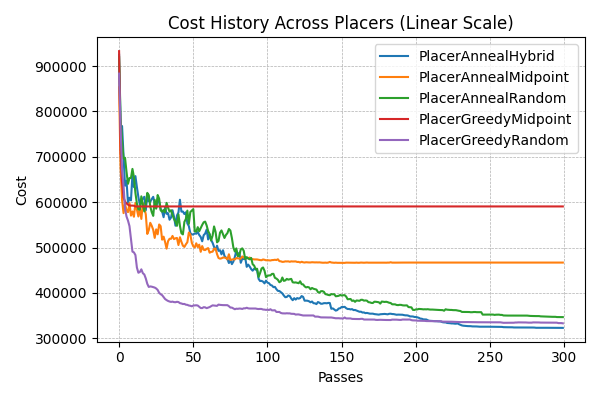
\includegraphics[width=\columnwidth]{figures/results/combined_cost_history_linear.png}
    \captionof{figure}{All placers overlaid}
    \label{fig:placers_overlay}
}


{
    \centering
    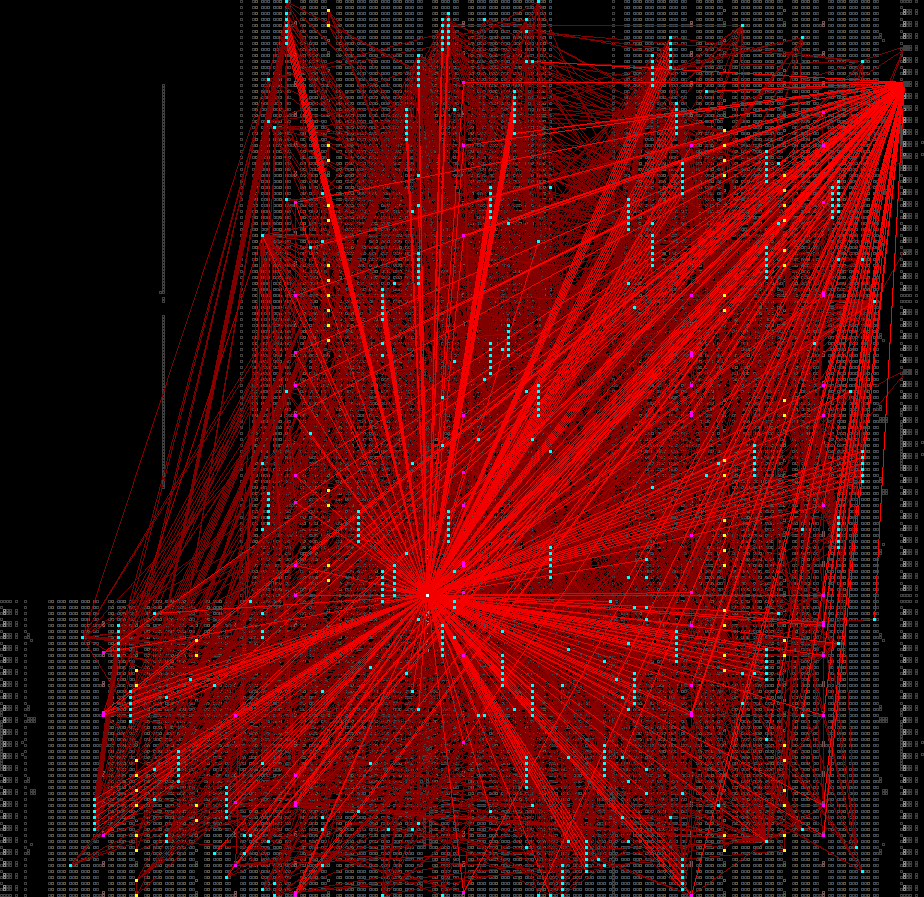
\includegraphics[valign=t, scale=0.13]{figures/results/PlacerGreedyRandom/random_placement.png}
    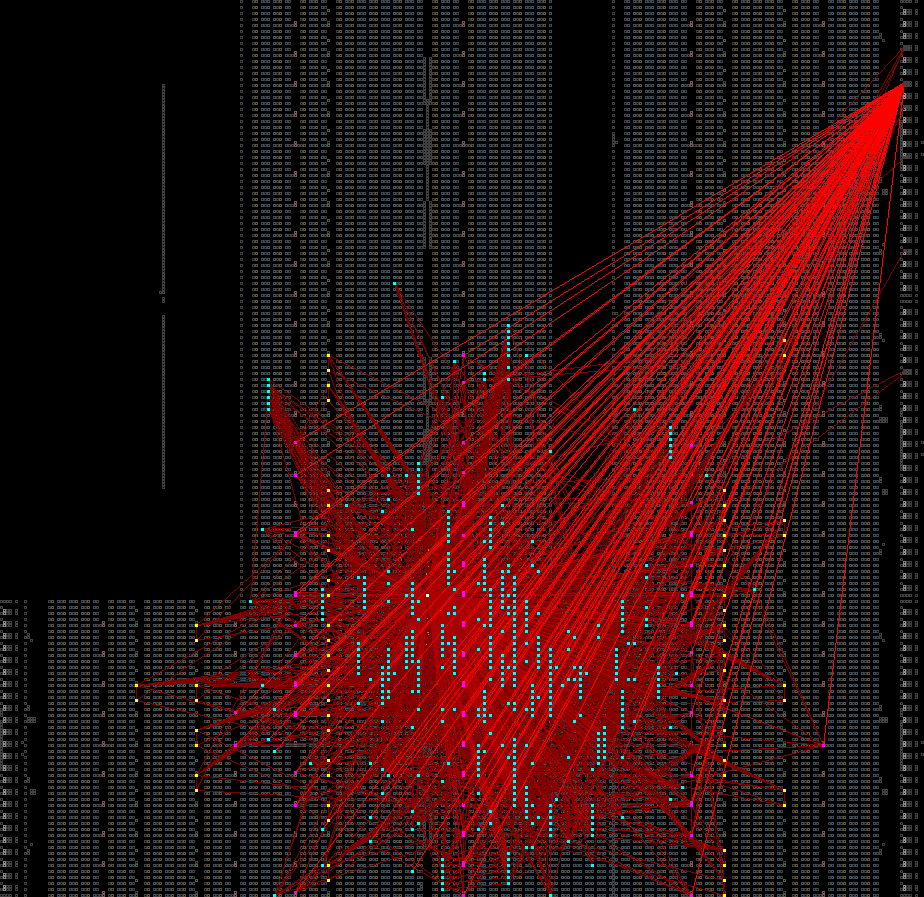
\includegraphics[valign=t, scale=0.13]{figures/results/PlacerGreedyRandom/00000010.png}
    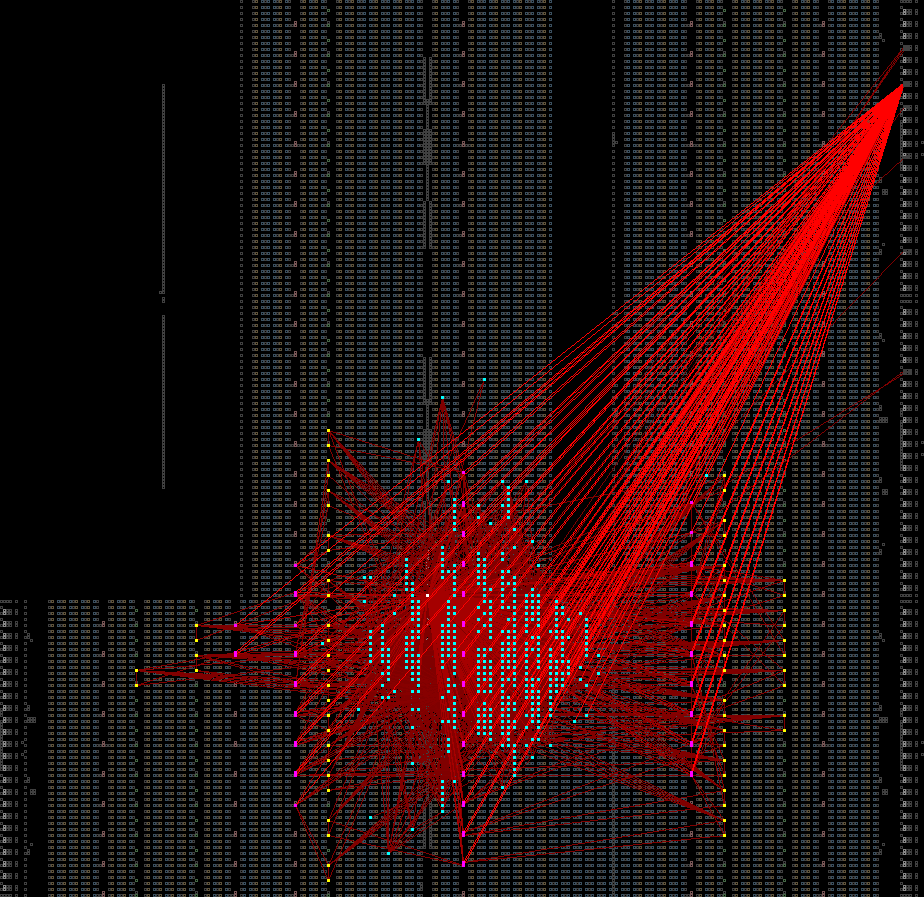
\includegraphics[valign=t, scale=0.13]{figures/results/PlacerGreedyRandom/00000100.png}
    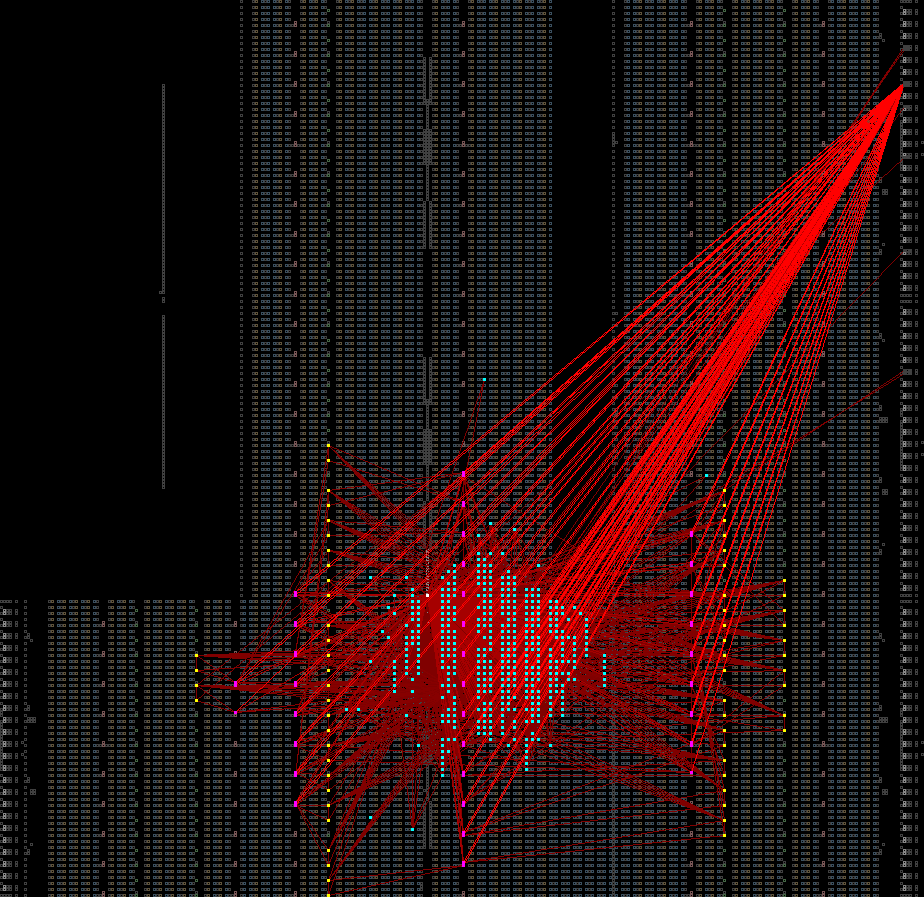
\includegraphics[valign=t, scale=0.13]{figures/results/PlacerGreedyRandom/00000299.png}
    \captionof{figure}{PlacerGreedyRandom}
    \label{fig:PGRSnapshots}
}

\columnbreak
{
    \centering
    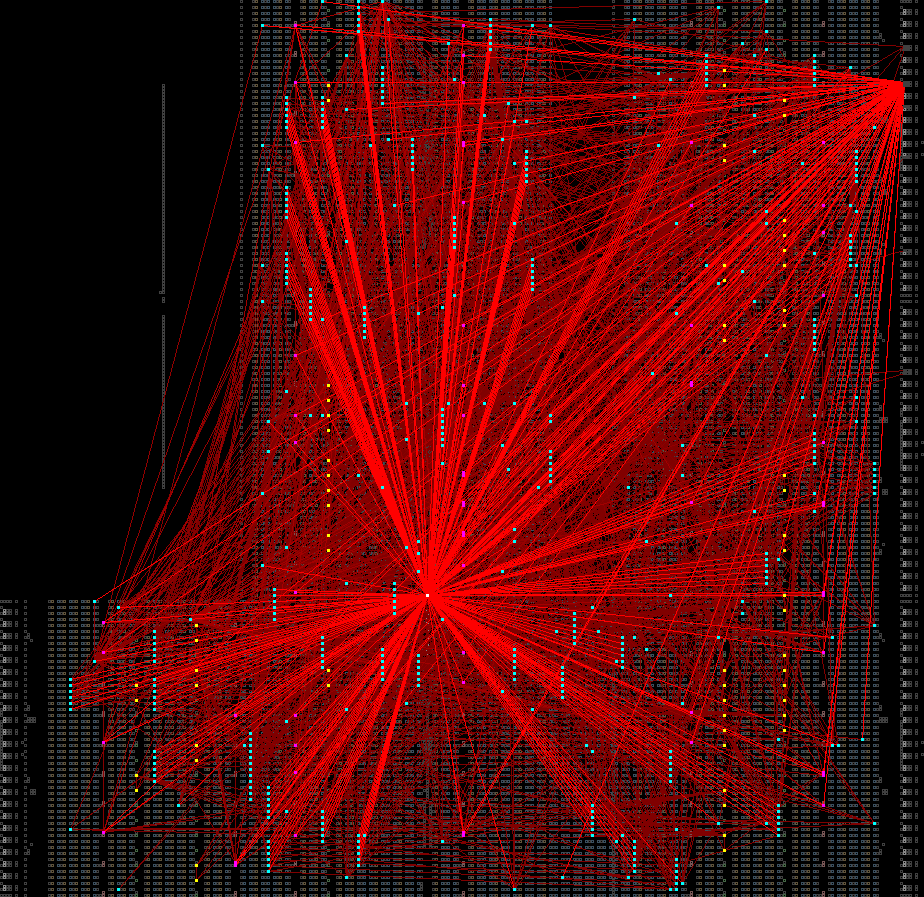
\includegraphics[valign=t, scale=0.13]{figures/results/PlacerGreedyMidpoint/random_placement.png}
    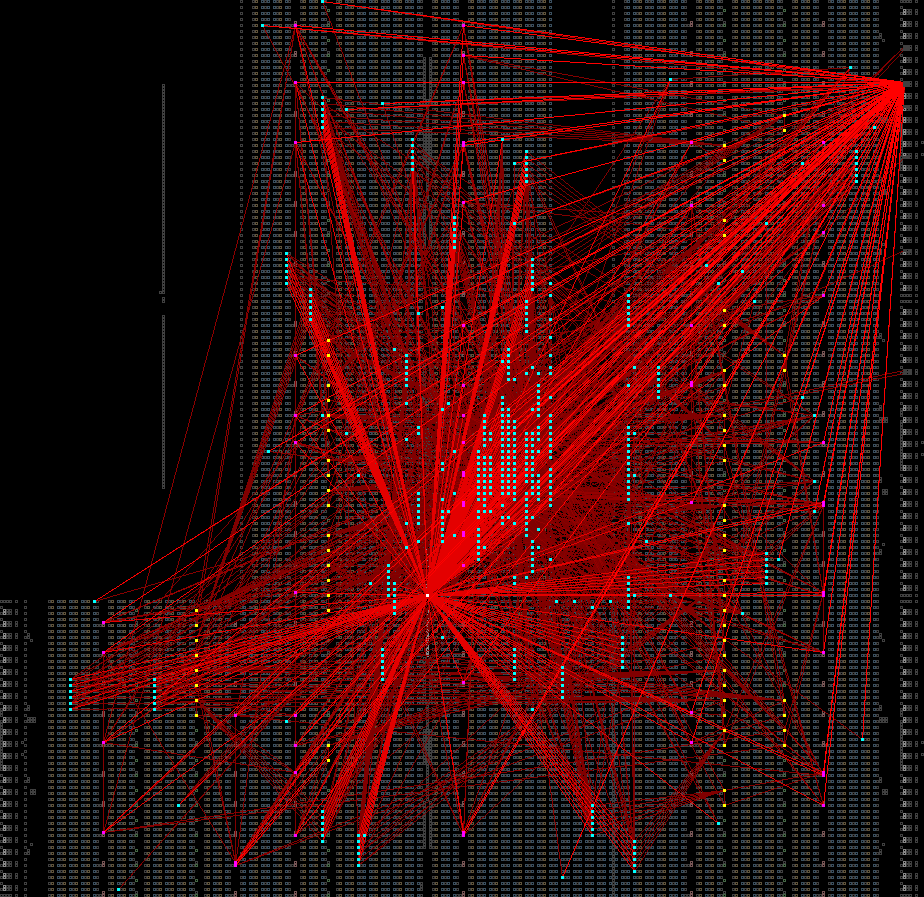
\includegraphics[valign=t, scale=0.13]{figures/results/PlacerGreedyMidpoint/00000010.png}
    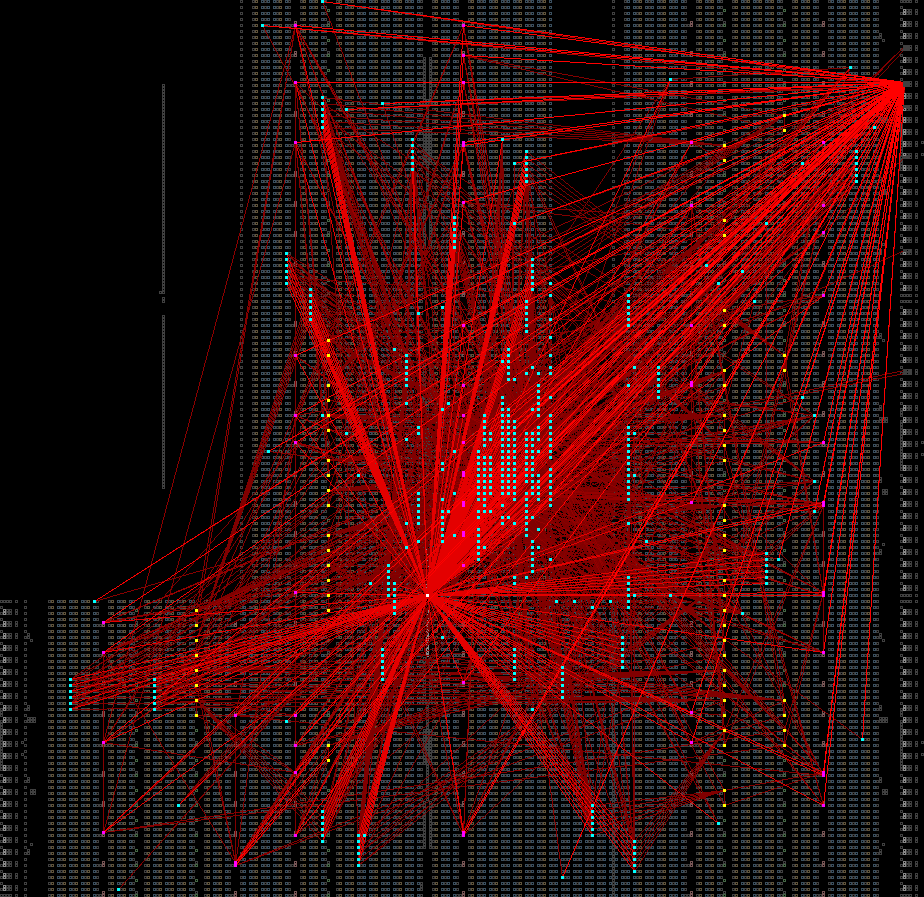
\includegraphics[valign=t, scale=0.13]{figures/results/PlacerGreedyMidpoint/00000100.png}
    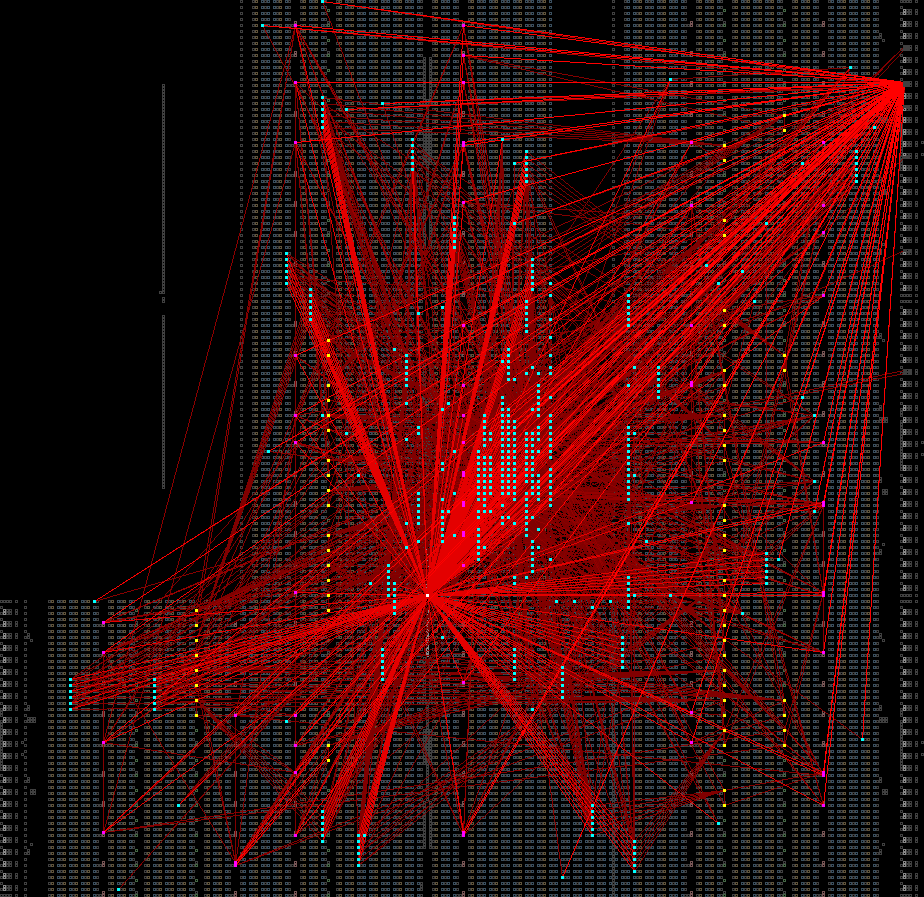
\includegraphics[valign=t, scale=0.13]{figures/results/PlacerGreedyMidpoint/00000299.png}
    \captionof{figure}{PlacerGreedyMidpoint}
    \label{fig:PGMSnapshots}
}
\vfill
{
    \centering
    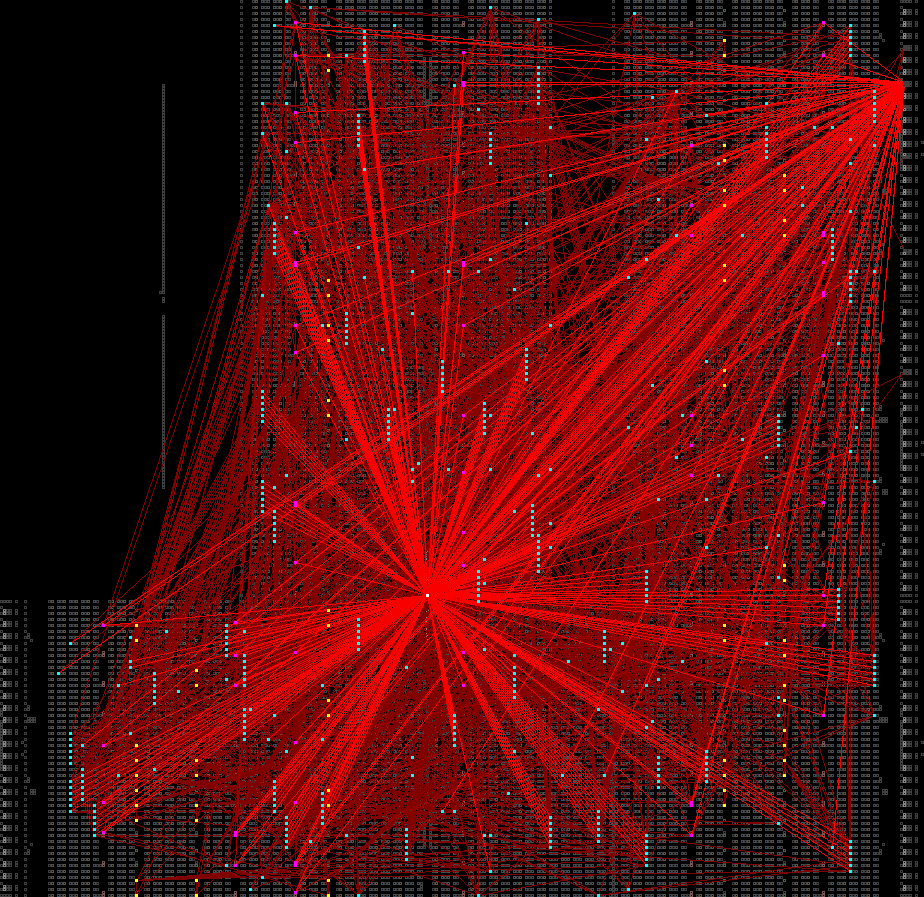
\includegraphics[valign=t, scale=0.13]{figures/results/PlacerAnnealRandom/random_placement.png}
    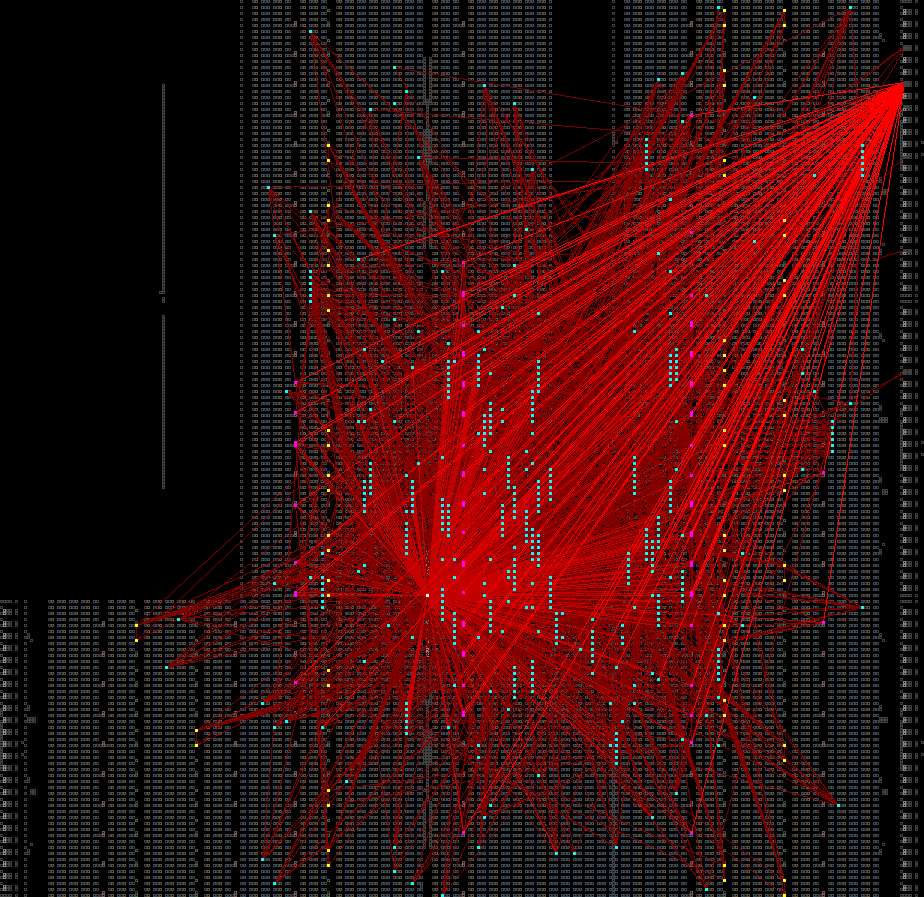
\includegraphics[valign=t, scale=0.13]{figures/results/PlacerAnnealRandom/00000010.png}
    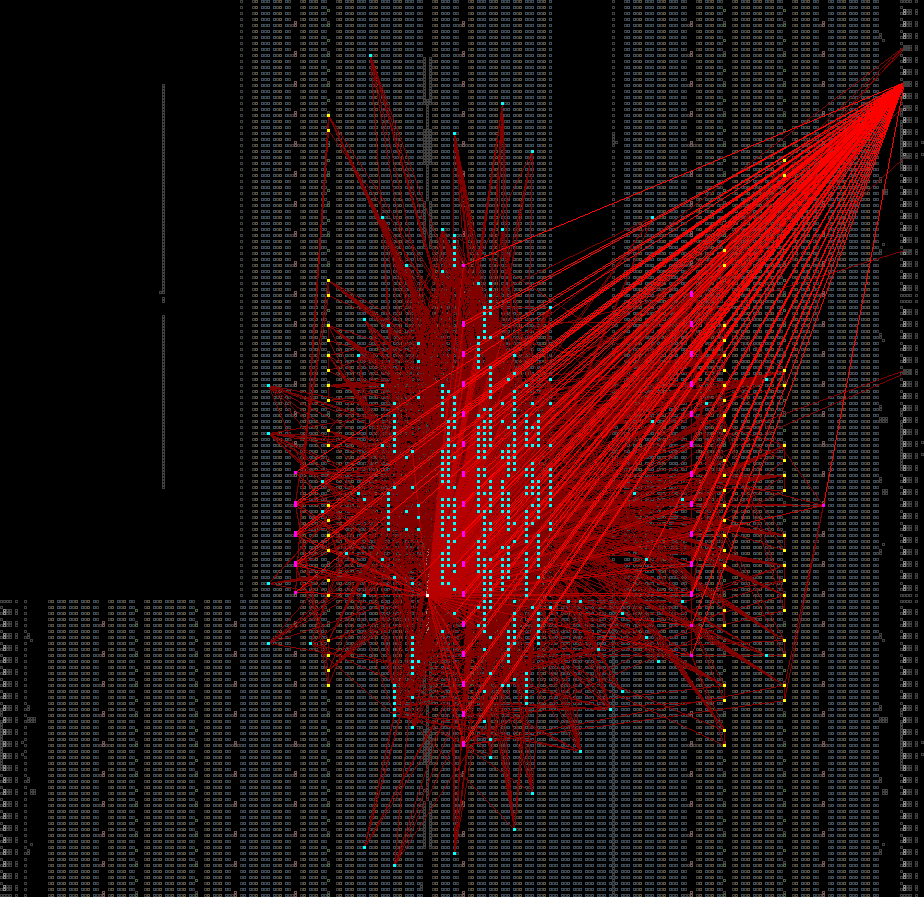
\includegraphics[valign=t, scale=0.13]{figures/results/PlacerAnnealRandom/00000100.png}
    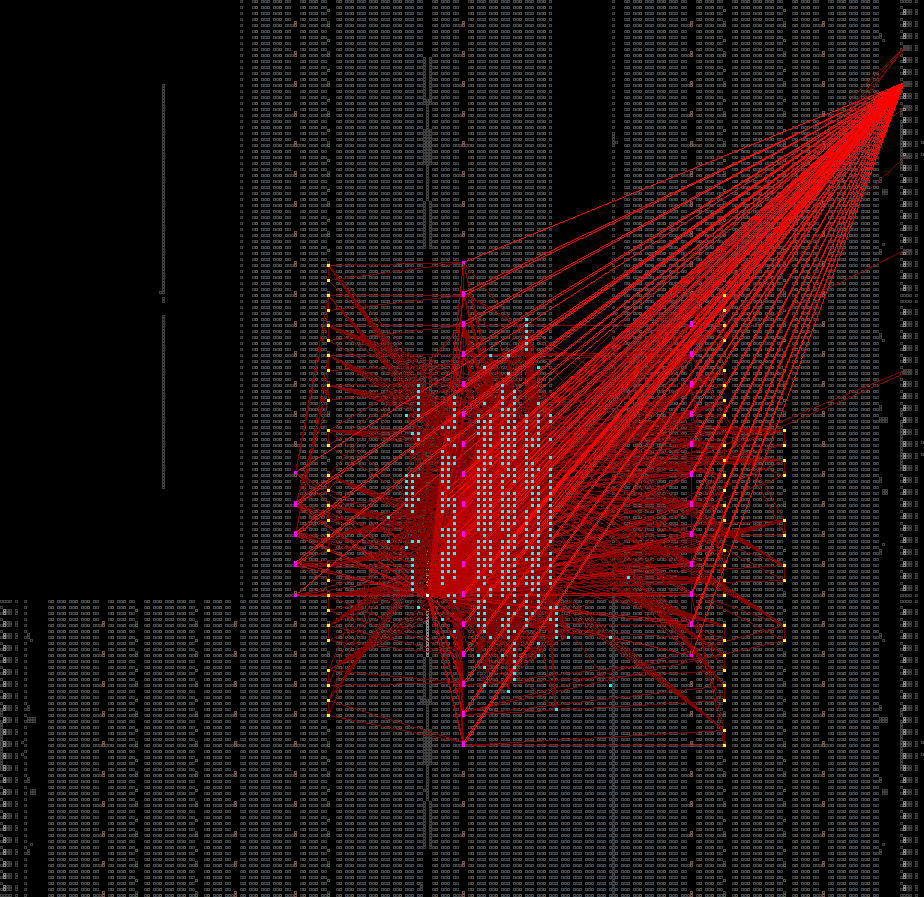
\includegraphics[valign=t, scale=0.13]{figures/results/PlacerAnnealRandom/00000299.png}
    \captionof{figure}{PlacerAnnealRandom}
    \label{fig:PARSnapshots}
}


\columnbreak
{
    \centering
    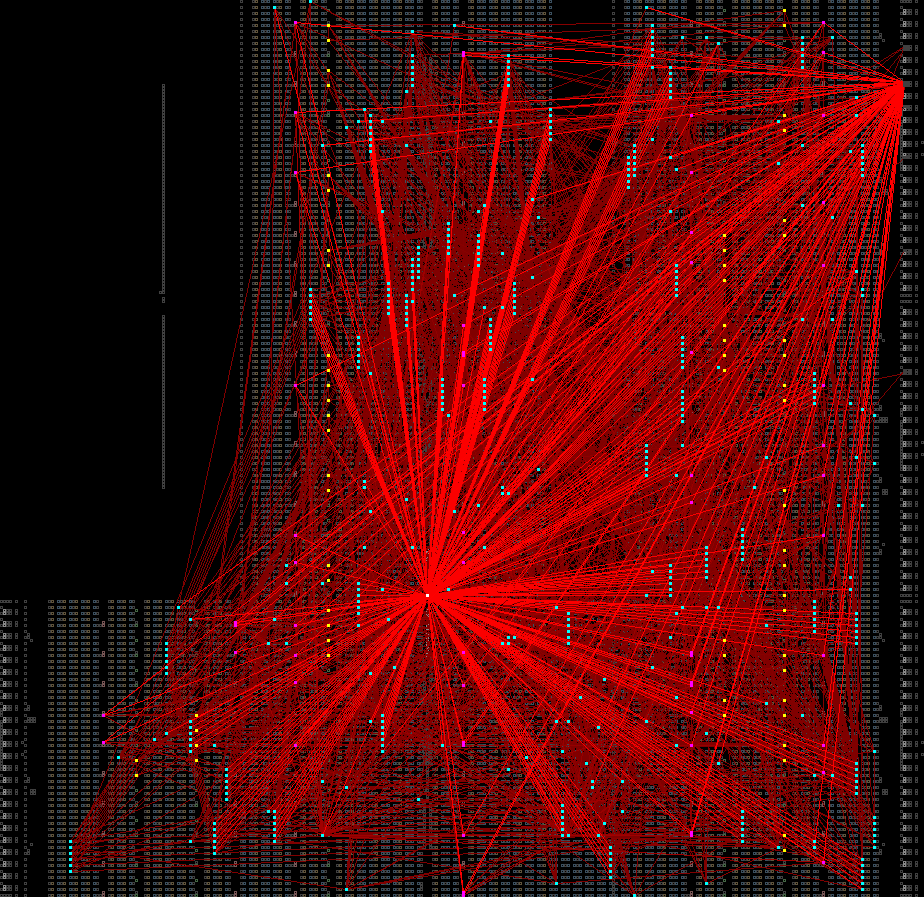
\includegraphics[valign=t, scale=0.13]{figures/results/PlacerAnnealMidpoint/random_placement.png}
    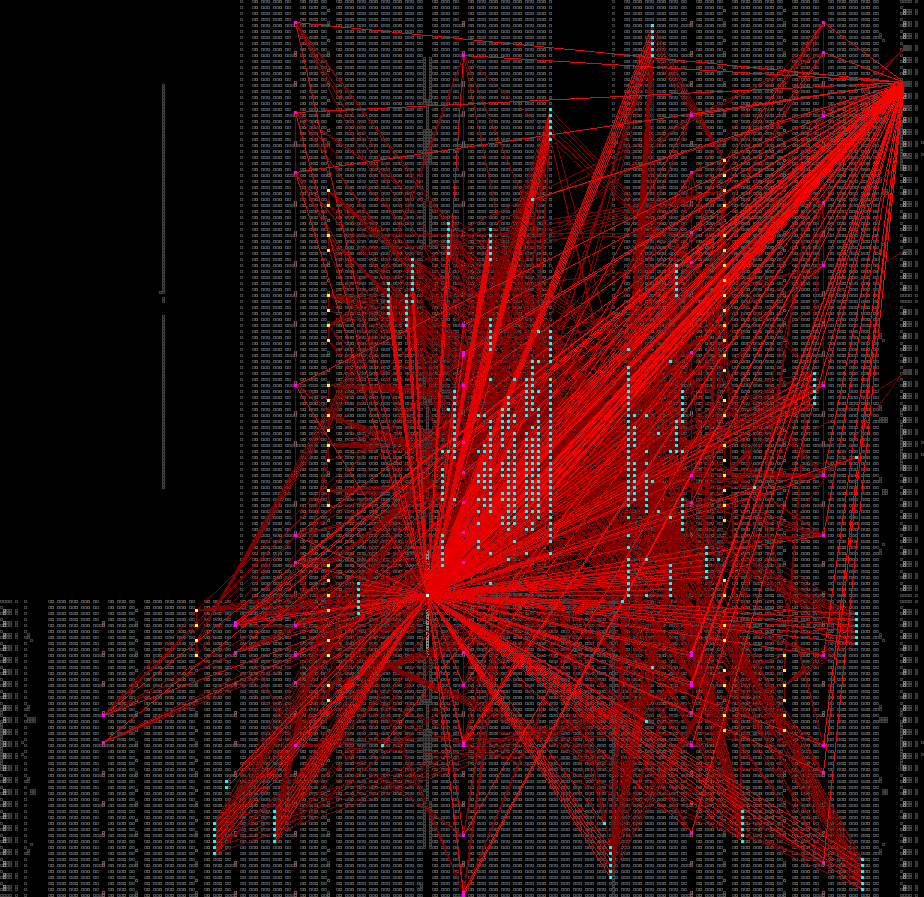
\includegraphics[valign=t, scale=0.13]{figures/results/PlacerAnnealMidpoint/00000010.png}
    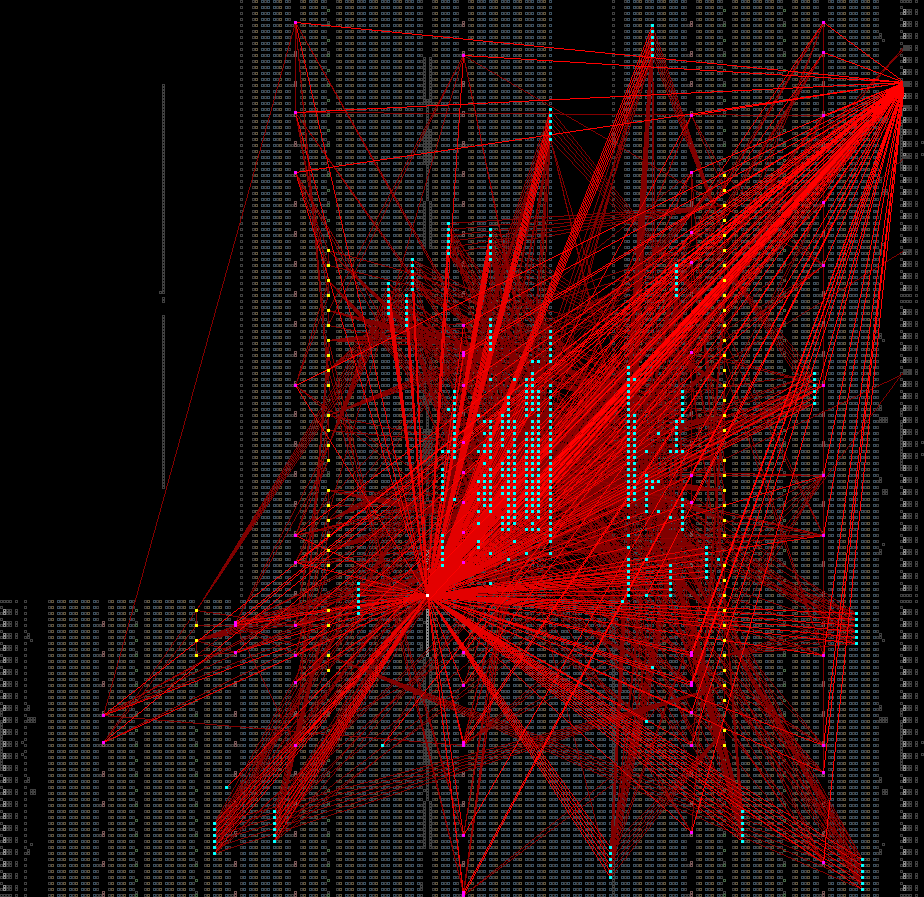
\includegraphics[valign=t, scale=0.13]{figures/results/PlacerAnnealMidpoint/00000100.png}
    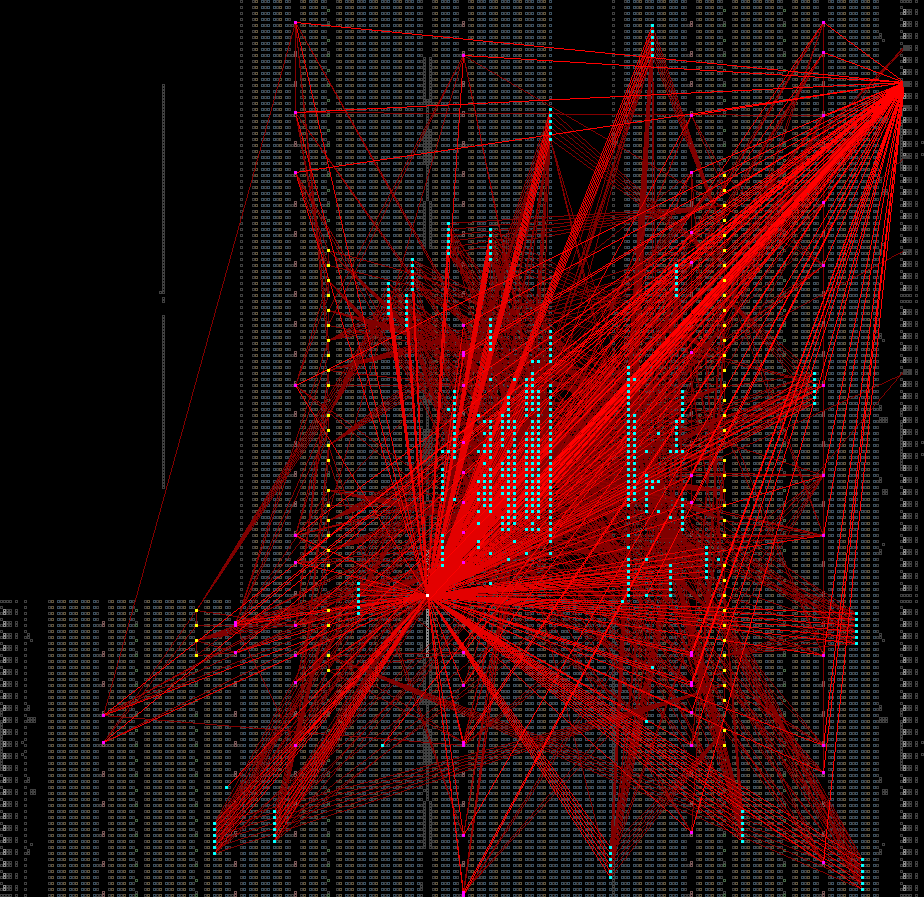
\includegraphics[valign=t, scale=0.13]{figures/results/PlacerAnnealMidpoint/00000299.png}
    \captionof{figure}{PlacerAnnealMidpoint}
    \label{fig:PAMSnapshots}
}
\vfill
{
    \centering
    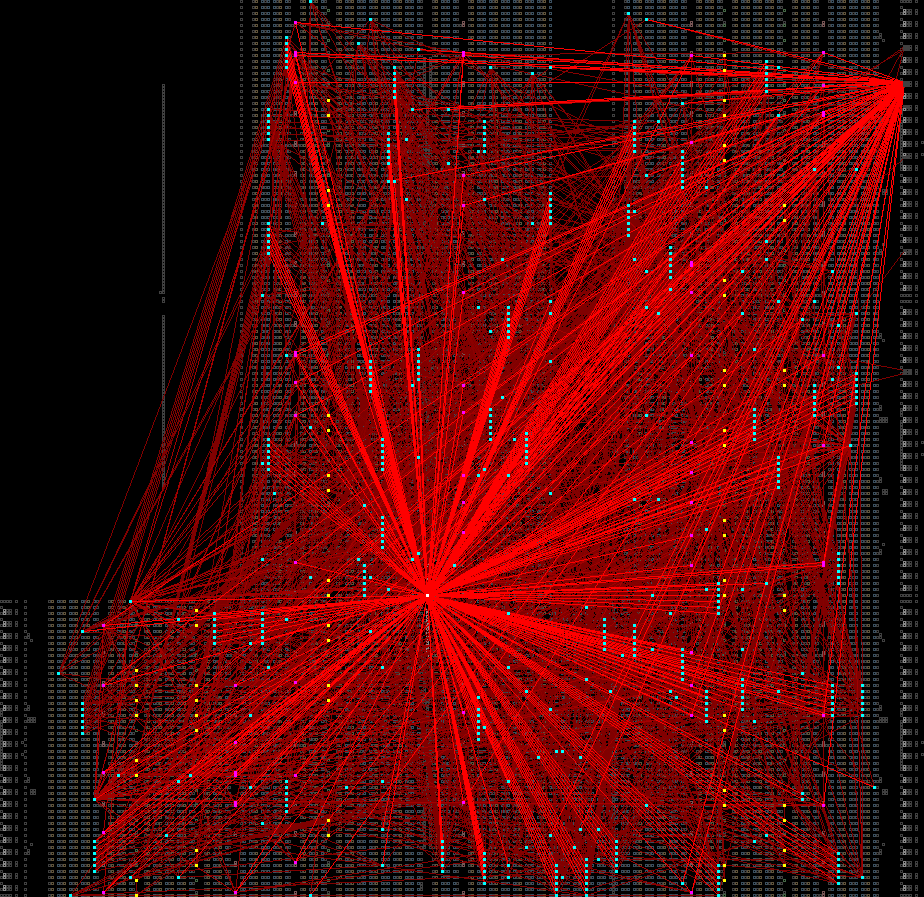
\includegraphics[valign=t, scale=0.13]{figures/results/PlacerAnnealHybrid/random_placement.png}
    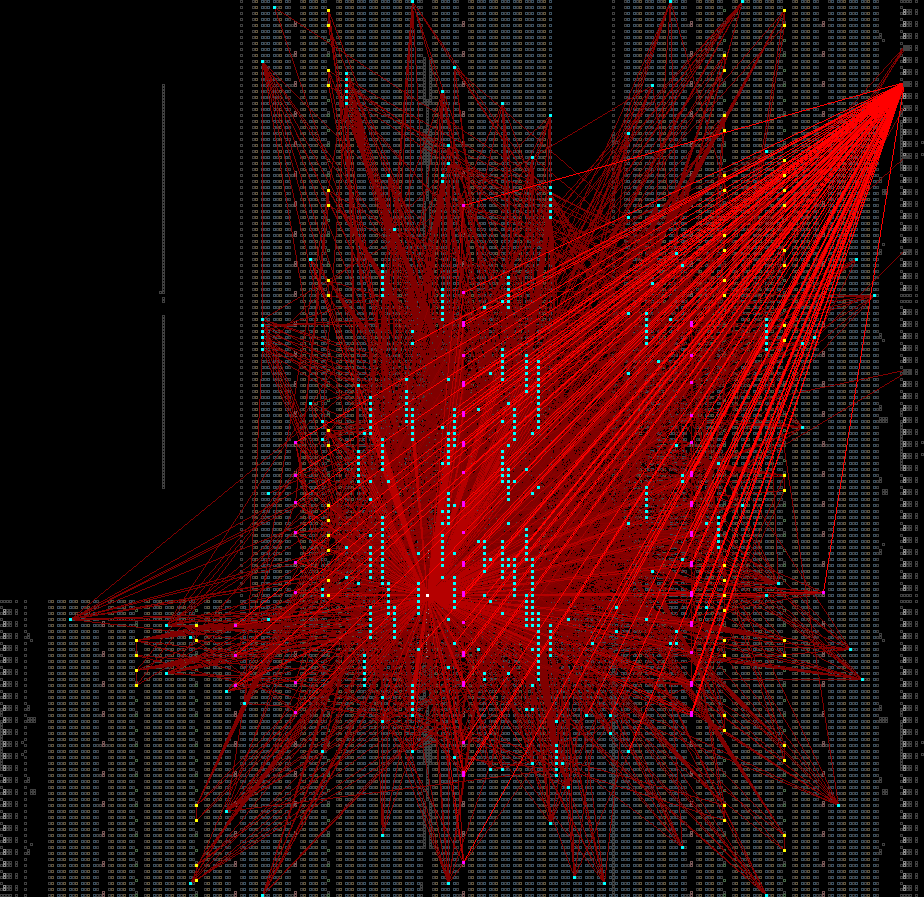
\includegraphics[valign=t, scale=0.13]{figures/results/PlacerAnnealHybrid/00000010.png}
    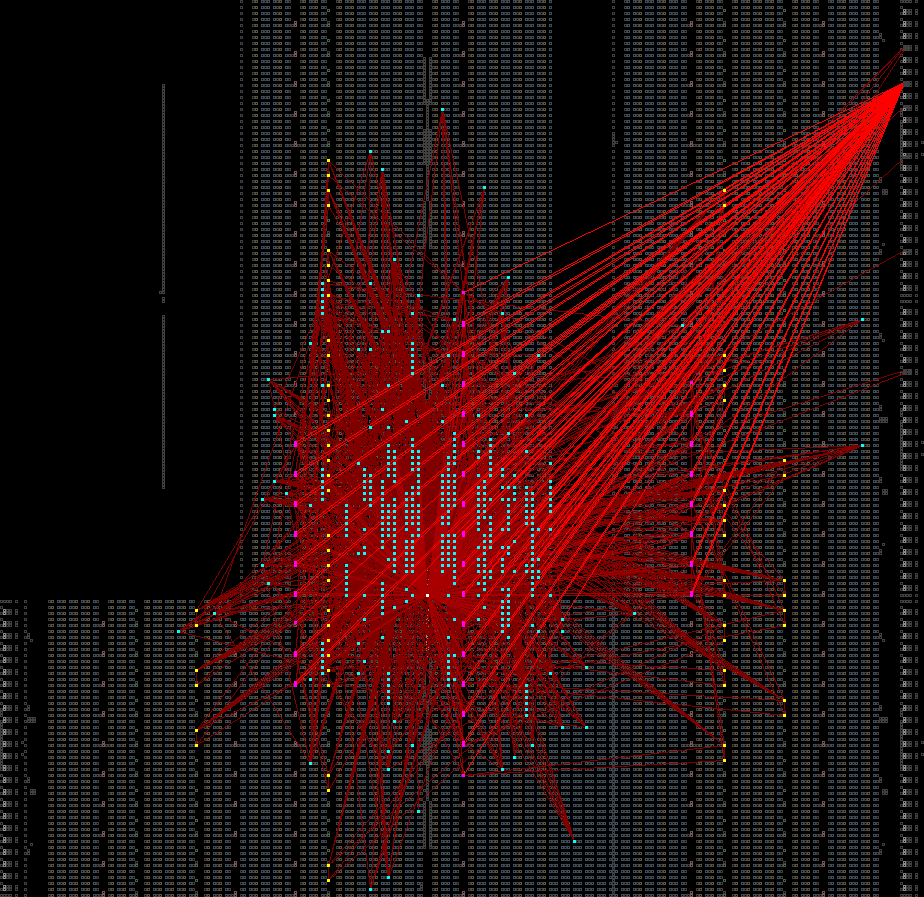
\includegraphics[valign=t, scale=0.13]{figures/results/PlacerAnnealHybrid/00000100.png}
    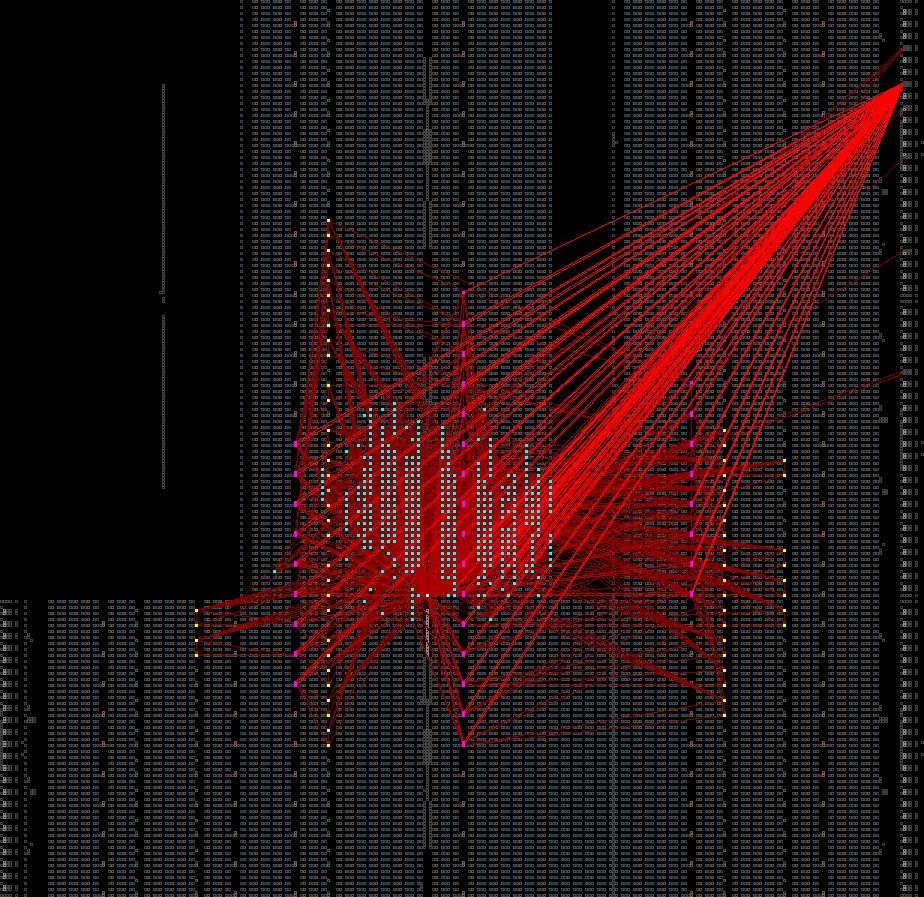
\includegraphics[valign=t, scale=0.13]{figures/results/PlacerAnnealHybrid/00000299.png}
    \captionof{figure}{PlacerAnnealHybrid}
    \label{fig:PAHSnapshots}
}


